\documentclass[journal,10pt]{IEEEtran}
\usepackage{hyperref}
\usepackage{todonotes}
\usepackage{amssymb}
\usepackage{amsmath}
\usepackage{mathtools}
\usepackage{graphicx}

\title{Predicting Parking Space Availability in Paderborn\\
Methodology Selection}
\author{Jan Lippert \(<\)\href{mailt:ljan@mail.upb.de}{ljan@mail.upb.de}\(>\)}
\date{\today}

\newcommand{\subtask}[1]{\begin{quote}\textbf{#1}\end{quote}}
\newcommand{\hod}{h}
\newcommand{\moh}{m}
\newcommand{\dow}{d}
\newcommand{\dom}{d_m}
\newcommand{\wom}{w_m}
\newcommand{\woy}{w_y}
\newcommand{\yyy}{a}

\newcommand{\IN}{\mathbb{N}}
\newcommand{\defeq}{\coloneqq}

\begin{document}
\maketitle

\section{Introduction}

In urban areas, space and as such parking space is limited. Car owners often have to drive around to available parking spots. This leads to an unnecessary waste of time and additional air pollution. 

According to multiple studies, the availability of parking data reduces the search time for a parking spot \cite{Asakura1994}\cite{Caicedo2010228}. However, most systems only provide the current number free parking spots. In rush hours, this information can quickly get outdated and lead to driving around to find available parking spaces.

The goal of this project is to predict the available parking space in advance. Because of the limitation outlined in \ref{sec:challenged}, we will focus on the covered car park ``Libori-Galerie''. This car park is also the most interesting as it is directly connected to a local shopping center. It is opened from 06:00 am to 02:00 am.
\section{Data Sources}\label{data sources}
The main data source is the actual parking data which is available online. In addition there are other possible features that may influence parking space availability. Since taking all features into account is not possible, this project will solely focus on the parking data in relation to time. 

\paragraph{Parking Usage Live Data}
The homepage of the ASP Paderborn\footnote{City-Managed service for waste management, city cleaning, and parking.} lists the city managed parking areas and the number of currently free parking spots. 
The data is available on \url{https://www.paderborn.de/microsite/asp/parken_in_der_city/freie_Parkplaetze_neu.php}. A more minimal website is available at \url{https://www4.paderborn.de/ParkInfoASP/default.aspx}. 

The website displays 4 attributes: name, type, capacity, and available spots\footnote{respectively: Parkstätte, --, Anzahl, Frei}. After crawling, the parking information will be annotated with the crawling time. The latter will be split into multiple attributes which will be used in the prediction: hour of day \(\hod\), minute of hour \(\moh\), day of week \(\dow\), day of month \(\dom\), week of month \(\wom\), week of year \(\woy\), and \(\yyy\)\footnote{the year is included as a way to keep samples unique in case the project runs more than 1 year.}.

The number of available parking spaces is be called \(y\). With the features defined before, the training data will be a set of tuples of the form  
\[
(\hod, \moh, \dow, \dom, \wom, \woy, \yyy, y)\text{.}
\]

\paragraph{Event Data (Optional)}
As mentioned in the first report, public holidays and local events could influence the parking situation near the city center. In some cases, these events take place \textit{on} one of the parking areas. However, as most of the big events do not happen while the course ``Practical Project in Machine Learning'' takes place, we will not consider them further.

\begin{figure}
  \centering
  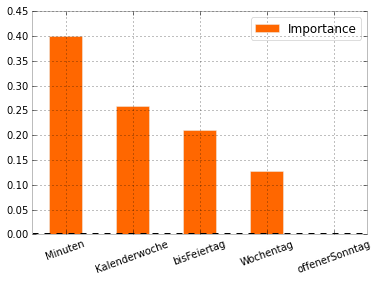
\includegraphics[scale=0.5]{parkendd-Feature-Importance.png}
  \caption{Importance of Features (ParkenDD)}
  \label{fig:parkendd_features}
\end{figure}

Public holidays like Christmas and Easter may also influence the availability of parking space. \cite[parkendd] modelled this in the feature ``bisFeiertag'', i.e. working days until public holiday. In figure \ref{fig:parkendd_features}, the relevance of the different features used by \cite{parkendd} is displayed\footnote{respectively: minutes, week of year, working days until public holiday, day of week, Sunday openings}. 

The feature was relatively important in the evaluation done by \cite{parkendd}. Nonetheless, it will not be included as the next public holiday is Christi Himmelfahrt on 25th May 2017. Therefore there would be no possibility of verifying the importance of this feature in time.

\paragraph{Weather Data (Optional)}

Weather data may also prove to be useful for prediction as, e.g., more people may decide to take the car when it's raining. Weather data is available online, e.g. at \url{https://openweathermap.org/api}. Weather data will not be considered in the prediction to keep the model simpler.


\section{Hypothesis}

It is assumed, that the available parking space is dependent on time, i.e. there exists a function \(f\) such that 
\[
f(\hod, \moh, \dow, \dom, \wom, \woy, \yyy) = y\text{.}
\]



\section{Feasibility}

To keep the scope of this project small, multiple data sources will be ignored. For this project, it is assumed that the number of available parking spots solely depends on time. As described in \ref{data sources}, this obviously is a very simplified model. However, as shown by \cite{parkendd}, such a simple model may be enough. 

The greatest challenge in this project is to collect enough training data to make meaningful predictions. All data needs to be extracted from APS's website. Changes to the website and non-availability of the service may prove problematic. In the beginning of February, the ASP parking guiding system was dysfunctional and did not show useful data online. 

The next limit is the usage of heroku's free plan. This plan limits the used database to 10000 rows. When crawling every 15 minutes, this limits the amount of available training data to roughly one week; the amount can be increased, since the 10000 row limit can be exceeded for 7 days before new inserts into the database are disabled.


\section{Model}
\subtask{Describe your selected model training method and discuss the reasoning behind your selection.}
\subsection{Training Methods} 

\section{Verification}
\subtask{Describe and discuss your ``objective method'', ie. the method by which you will measure the success of your predictor.}
To verify the trained model and the accuracy of its predictions, the predictions will be queried in regular intervals and compared to the actual available parking space at that time. 


\bibliographystyle{ieeetr}  
\bibliography{report_2}

\end{document}
